\documentclass{article}

\usepackage[utf8]{inputenc}  
\usepackage[T1]{fontenc}     
\usepackage{tikz}
\usetikzlibrary{shapes, positioning, arrows, calc}
\usetikzlibrary{decorations.pathreplacing}

\begin{document}

% Exemple tri

% tour 1

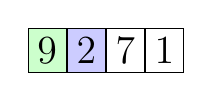
\begin{tikzpicture}
   \node [fill=green!20, font=\sffamily\Large\bfseries, draw, anchor=center] (first) {$9$};
   \node [fill=blue!20, font=\sffamily\Large\bfseries, draw, anchor=center, right=0cm of first] (second) {$2$};
   \node [font=\sffamily\Large\bfseries, draw, anchor=center, right=0cm of second] (third) {$7$};
   \node [font=\sffamily\Large\bfseries, draw, anchor=center, right=0cm of third] (fourth) {$1$};
\end{tikzpicture}

% tour 2

\vspace{1cm}

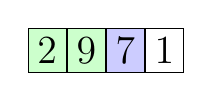
\begin{tikzpicture}
   \node [fill=green!20, font=\sffamily\Large\bfseries, draw, anchor=center] (first) {$2$};
   \node [fill=green!20, font=\sffamily\Large\bfseries, draw, anchor=center, right=0cm of first] (second) {$9$};
   \node [fill=blue!20, font=\sffamily\Large\bfseries, draw, anchor=center, right=0cm of second] (third) {$7$};
   \node [font=\sffamily\Large\bfseries, draw, anchor=center, right=0cm of third] (fourth) {$1$};
\end{tikzpicture}

% tour 3

\vspace{1cm}

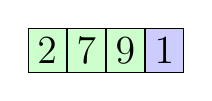
\begin{tikzpicture}
   \node [fill=green!20, font=\sffamily\Large\bfseries, draw, anchor=center] (first) {$2$};
   \node [fill=green!20, font=\sffamily\Large\bfseries, draw, anchor=center, right=0cm of first] (second) {$7$};
   \node [fill=green!20, font=\sffamily\Large\bfseries, draw, anchor=center, right=0cm of second] (third) {$9$};
   \node [fill=blue!20, font=\sffamily\Large\bfseries, draw, anchor=center, right=0cm of third] (fourth) {$1$};
\end{tikzpicture}

% tour 4

\vspace{1cm}

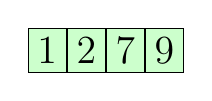
\begin{tikzpicture}
   \node [fill=green!20, font=\sffamily\Large\bfseries, draw, anchor=center] (first) {$1$};
   \node [fill=green!20, font=\sffamily\Large\bfseries, draw, anchor=center, right=0cm of first] (second) {$2$};
   \node [fill=green!20, font=\sffamily\Large\bfseries, draw, anchor=center, right=0cm of second] (third) {$7$};
   \node [fill=green!20, font=\sffamily\Large\bfseries, draw, anchor=center, right=0cm of third] (fourth) {$9$};
\end{tikzpicture}

\end{document}
